\section{Index and B+ Trees} 

  So far, we've abstracted away the inner workings of the DBMS and was just told to trust it. From here, we'll delve into the inner workings of modern DBMS systems, starting with hardware.   

\subsection{Hardware and Memory Layout}

  Recall the memory hierarchy, which starts with CPU registers, followed by caches, memory, and a disk. The speed of read/write, called I/O, determines how fast you can retrieve this data. 

  \begin{definition}[Hard Disk]
    In SQL queries, the (disk) I/O dominates the execution time, so this must be analyzed first. A typical hard drive consists of a bunch of \textbf{disks/platters} that are spun by a \textbf{spindle} and read by a \textbf{disk head} on a \textbf{disk arm}. Each disk is pizza sliced into \textbf{sectors} and donut sliced into \textbf{tracks} (and a collection of tracks over all disks is a \textbf{cylinder}), and the arm will read one \textbf{block} of information, which is a logical unit of transfer consisting of one or more blocks (i.e. like a word, which is usually 4 bytes).\footnote{You cannot just write 1 byte. You must rewrite the entire block with the 1 byte updated. If we want to write 2 bytes which are on separate blocks, we must do 2 block writes.} 
  \end{definition}

  \begin{definition}[Access Time]
    The access time is the sum of 
    \begin{enumerate}
      \item the \textit{seek time}: time for disk heads to move to the correct cylinder 
      \item the \textit{rotational delay}: time for the desired block to rotate under the disk head 
      \item the \textit{transfer time}: time to read/write data on the block
    \end{enumerate}
    This spindle rotation and moving arm is slow, so the times are dominated by the first two. 
  \end{definition}

  Note that this is heavily dependent on the data being accessed. Sequential data is extremely fast while random access is slow. Therefore, we should try to store data that should be accessed together next to each other in the disk.  

  \begin{definition}[Memory, Buffer Pool]
    As we expect, the DBMS stores a cache of blocks, called the \textbf{memory/buffer pool} containing some fixed size of $M$ maximum blocks. We read/write to this pool of blocks (which costs some time per blocks) and then these dirty (which are written/updated) are flushed back to the disk. It essentially acts as a middleman between the disk and the programmers, and every piece of data that goes between the two must go through the memory. 

    \begin{figure}[H]
      \centering 
      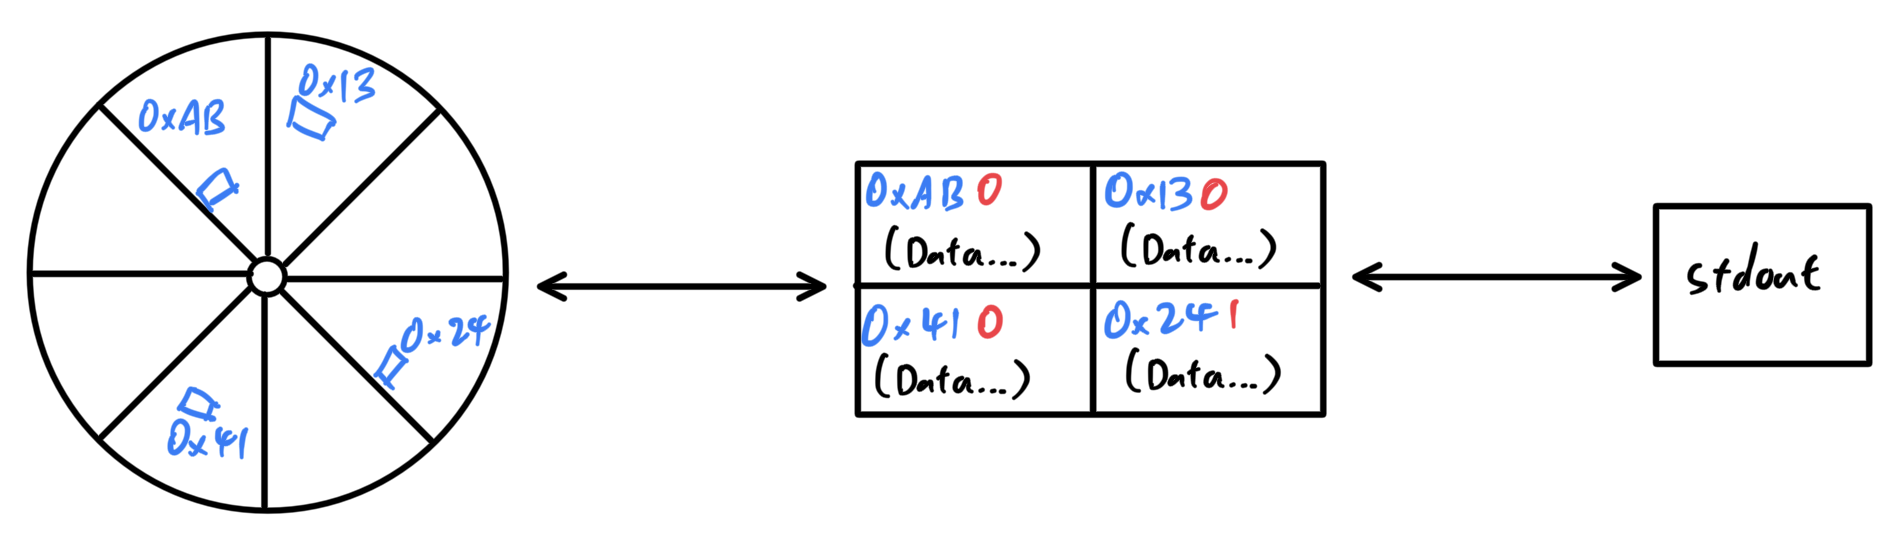
\includegraphics[scale=0.4]{img/disk_memory.png}
      \caption{We store the memory address of the block (blue) and a bit indicating whether it is dirty or not (red). } 
      \label{fig:disk_memory}
    \end{figure}
  \end{definition}

  Therefore, if we want to read $N > M$ blocks, then the first $M$ blocks must be loaded into memory, outputted into stdout, and then the memory must be refilled with the rest of the blocks. If we have updated a block in memory, then we should flush it before overwriting this block in memory.\footnote{idk perhaps we can have a overhead bit indicating whether a block is updated, along with the memory address of this block so it can find it back on the disk.} Replacement strategies won't be covered here. Note that unlike algorithms, which focus on the cost of the algorithm after it is read into memory, we focus on the cost of loading data from the disk into memory. 

  So how should we increase performance? 
  \begin{enumerate}
    \item \textit{Disk Layout}: Keep related things close together, e.g. in the same sector/block, or same track, or same cylinder, or adjacent cylinders. 
    \item \textit{Prefetching}: When fetching a block from the disk, fetch the next block as well since it's pretty likely to access data from the next block. This is basically locality. 
    \item \textit{Parallel I/O}: We can have more heads working at the same time. 
    \item \textit{Disk Scheduling Algorithm}: e.g. the elevator algorithm sorts the cylinders so that you don't go back and forth between cylinders when fetching.  
    \item \textit{Track Buffer}: Read/write one entire track at a time. 
  \end{enumerate}

  Now let's talk about how the actual bytes are stored in memory. 

  \begin{definition}[Row Major Order, NSM]
    We group rows together contiguously in the disk block.\footnote{This is the most standard storage policy.} If we have a relation with schema \texttt{R(INT(4), CHAR(24), INT(4), DOUBLE(8))}, we first store the rows together, with extra space in between since we might append new attributes, and have a tuple of pointers to the start of each row (orange lines). 

    \begin{figure}[H]
      \centering 
      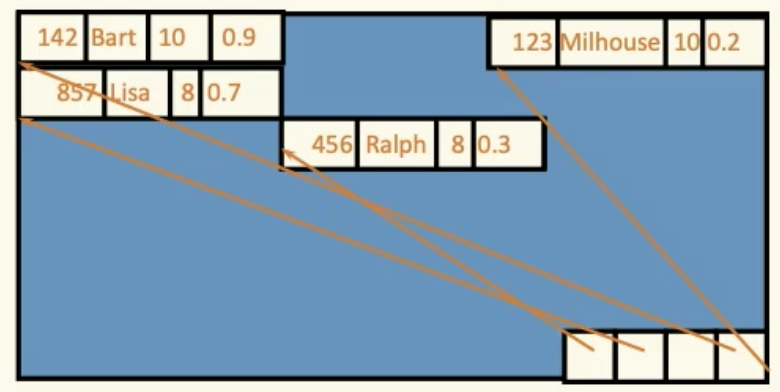
\includegraphics[scale=0.6]{img/row_major.png}
      \caption{} 
      \label{fig:row_major.png}
    \end{figure}
  \end{definition}

  Note that \texttt{VARCHAR} still allocates the same number of bytes, but adds padding. 

  \begin{definition}[Column Major, PAX]
    We group columns together contiguously in the disk block, which allows for optimization since all types are the same and we can just use pointer arithmetic to get every attribute in $O(1)$ time. We split the block into chunks and have metadata of pointers that point to the start of the array for each attribute. 

    \begin{figure}[H]
      \centering 
      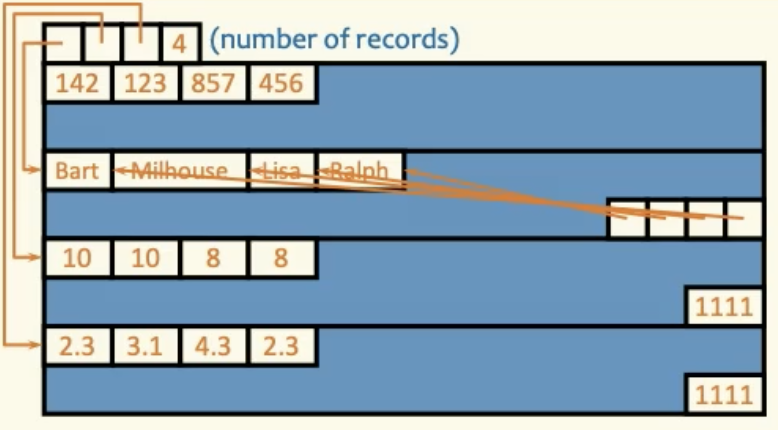
\includegraphics[scale=0.6]{img/column_major.png}
      \caption{} 
      \label{fig:column_major}
    \end{figure}
  \end{definition}

\subsection{Search Keys and Index} 

  Now that we've seen how the data is actually laid out in memory, we can look under the hood to see what happens when we make a query as such. Consider the relation schema \texttt{User(\underline{uid}, age)}, along with the two SQL queries, specifying on the key attribute and a non-key attribute. 
  
  \noindent\begin{minipage}{.5\textwidth}
    \begin{lstlisting}[]{Code}
      SELECT * 
      FROM User 
      WHERE uid = 112;
    \end{lstlisting}
    \end{minipage}
    \hfill
    \begin{minipage}{.49\textwidth}
    \begin{lstlisting}[]{Output}
      SELECT * 
      FROM User 
      WHERE age = 12;
    \end{lstlisting}
  \end{minipage} 

  The DBMS will have to go to disk and scan it to find the tuples satisfying the predicate. However, it is a bit more sophisticated than a simple complete scan. 

  \begin{definition}[Search Key]
    The \textbf{search key} is simply the attribute on which our query is defined (e.g. \texttt{uid} and \texttt{age} in the example above). The values (e.g. \texttt{112} and \texttt{12}) are called the \textbf{search key values}. 
  \end{definition} 

  This is distinct from a closely-related concept called the index, which also refers to attributes. The tuples may take on some structure depending on the attribute. It may be sorted in one attribute but random in another. 

  \begin{definition}[Index]
    This set of attribute values, which really act as pointers, that we use to scan more efficiently on disk is called the \textbf{index}. 

    \begin{figure}[H]
      \centering 
      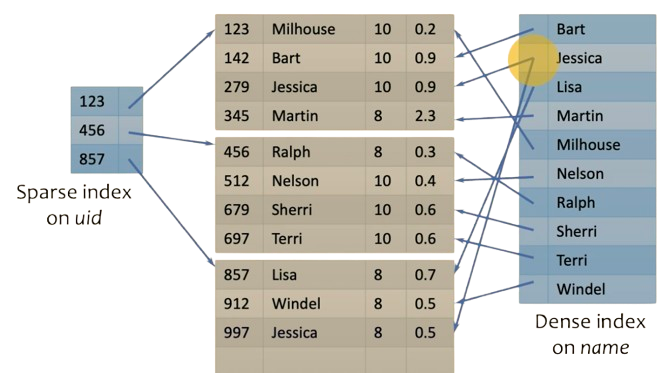
\includegraphics[scale=0.4]{img/dense_sparse.png}
      \caption{The dense index has 10 values, but there are two Jessicas, so it is indeed dense. The sparse index is on the uid, and since the relation is sorted (a more specific form of \textit{clustering}) in the disk, we can use sparse keys.} 
      \label{fig:dense_sparse}
    \end{figure}

    Sparse and dense just refers to how much an index ``covers'' a disk block. 
    \begin{enumerate}
      \item A \textbf{dense index} means that there is one index entry for each search key value. One entry may point to multiple records
      \item A \textbf{sparse index} means that there is one index entry for each block. Records must be clustered according to the search key as shown below, and this can optimize searching. 
    \end{enumerate}

    Note that 
    \begin{enumerate}
      \item The sparse index must contain at least the number of blocks, while the dense index must contain at least the number of unique search key values. Since the sparse index is much smaller, we may be able to fit it into main memory and not have to pay the I/O cost. 
      \item A dense index does not require anything on the records, while the sparse requires the data to be clustered. 
      \item Lookup is easy on dense since we can directly see if it exists. For sparse, we must first follow the pointer and scan the block. (e.g. if we wanted to look for 279, we want to look at the address pointed to by 123, and scan down until we hit it or reach a number greater than 279). 
      \item Update is usually easier on sparse indices since we don't need to update the index unless we add a new block. For dense, if we added a new person Muchang, then we would have to add \texttt{Muchang} to the dense index. 
    \end{enumerate}
  \end{definition}

  \begin{definition}[Primary vs Secondary Index]
    Primary and secondary refers to what the index is over. 
    \begin{enumerate}
      \item A \textbf{primary index} is created for the primary key of the relation. Records are usually clustered by the primary key, so this can be sparse. 
      \item A \textbf{secondary index} is any index that is not over a primary key and is usually dense. 
    \end{enumerate}
    In SQL, the \texttt{PRIMARY KEY} declaration automatically creates a primary index, and the \texttt{UNIQUE} declaration creates a secondary index. 
  \end{definition}

  \begin{example}[Additional Secondary Indices]
    You can also create an additional secondary index on non-key attributes. For example, if you think that you will query based on popularity often, you can do 
    \begin{lstlisting}
      CREATE INDEX UserPopIndex ON User(pop); 
    \end{lstlisting}
    which will create a dense index to speed up lookup at the cost of memory. 
  \end{example}

\subsection{Tree Index} 

  \subsubsection{B-Trees}

    So really, an index is really a set of pointers, but we must be able to store this set of pointers. This leads to the problem of the index being too big to fit into a block. In this case, we can just create a sparse index on top of the dense index. This allows us to store a large index across blocks. 
    
    \begin{figure}[H]
      \centering 
      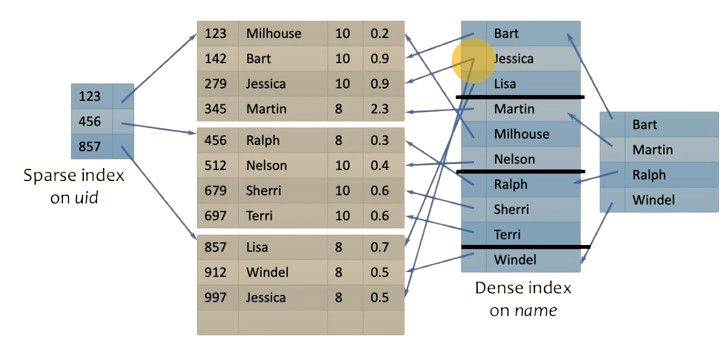
\includegraphics[scale=0.4]{img/too_big.png}
      \caption{We store a sparse index in memory which points to a dense index on disk, which then points to the tuples of the relation, also on disk. } 
      \label{fig:too_big}
    \end{figure}

    If the index is still too big, we store another index on top of that, and we have pretty much a tree. This is called the Index Sequential Access Method (ISAM). 
    
    \begin{example}[Index Traversal in Tree]
      If we want to look up 197 in this tree, we traverse down. Note that we have the root node in memory already, but we would require an IO operation to traverse the pointer to the first block, and then another IO cost to go to the second. 
      \begin{figure}[H]
        \centering 
        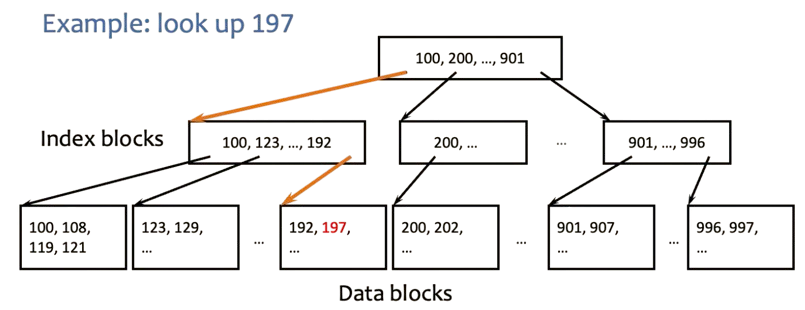
\includegraphics[scale=0.4]{img/isam_lookup.png}
        \caption{An index tree of depth 3.} 
        \label{fig:isam_lookup}
      \end{figure}
    \end{example}

    A problem with this method is also a problem with BSTs. If we want to delete 123 and add 107 ten times, then we have an unbalanced binary search tree and in extreme cases, this reduces to a linear search. 

    \begin{figure}[H]
      \centering 
      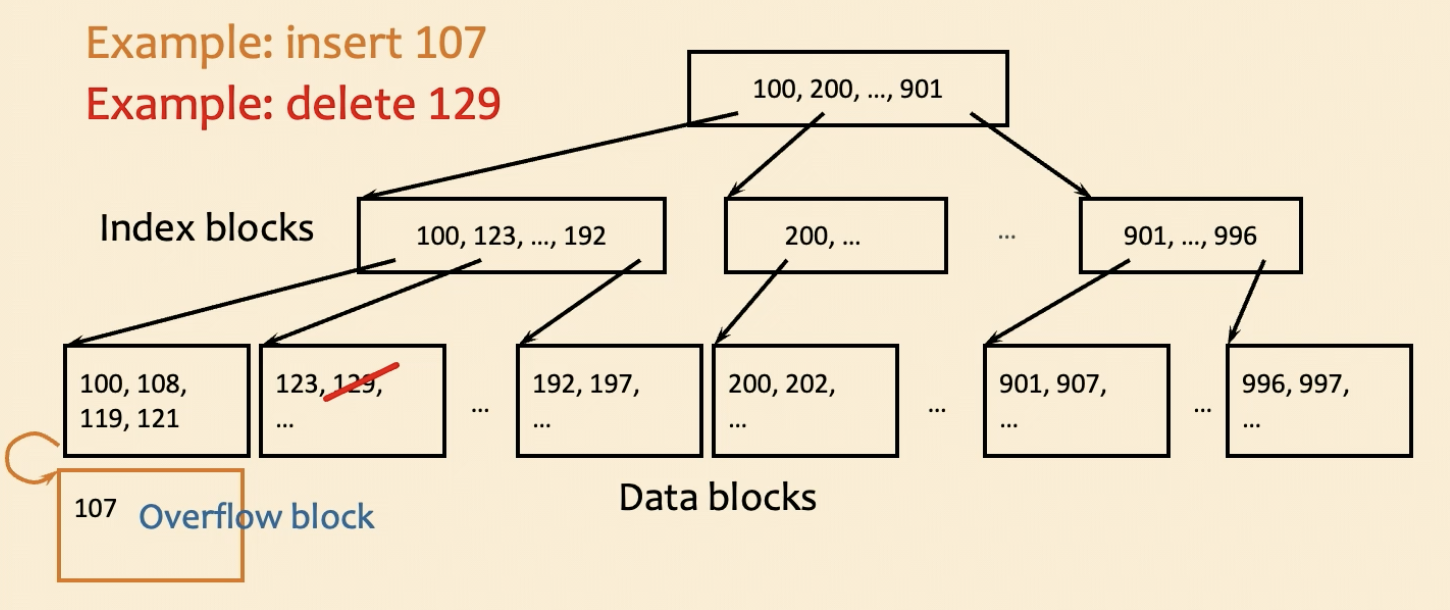
\includegraphics[scale=0.4]{img/isam_problem.png}
      \caption{If this block overflows, then we want to expand this, leading to an unbalanced BST and reducing our search to linear time.} 
      \label{fig:isam_problem}
    \end{figure}
    

    \begin{definition}[B Tree]
      Therefore, this static data structure is not good, and we must use a more flexible one, called a \textbf{B-tree}.
      \begin{figure}[H]
        \centering 
        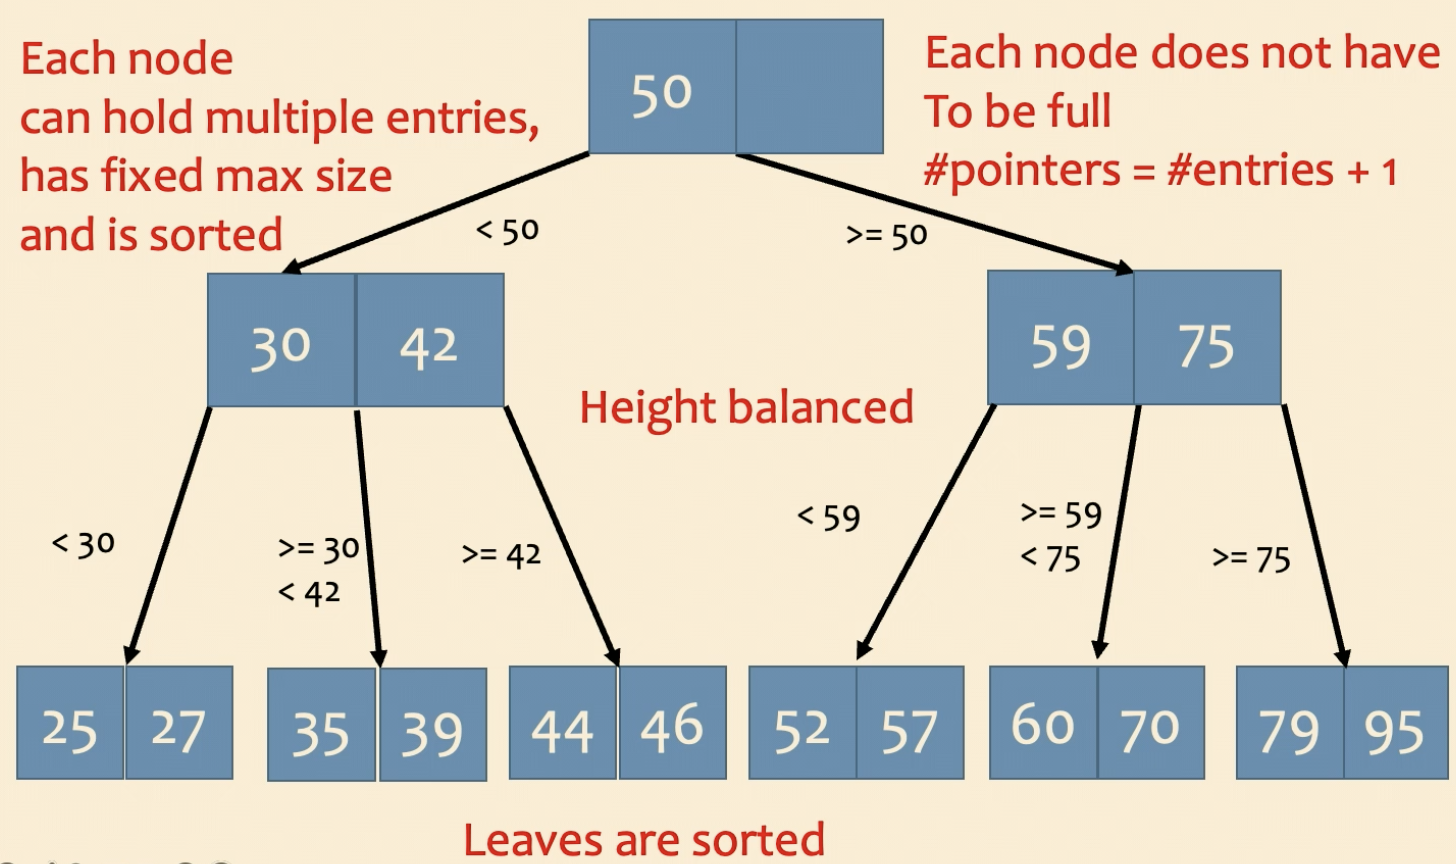
\includegraphics[scale=0.4]{img/b_tree.png}
        \caption{B-tree. Each node can now hold multiple entries in sorted order. It is height balanced, though we will not show it here.} 
        \label{fig:b_tree}
      \end{figure}
    \end{definition}

  \subsubsection{B+ Trees}

    The actual structure that modern DBMS uses is the slightly more sophisticated B+ tree. 

    \begin{definition}[B+ Tree]
      While in B trees, the non-leaf nodes are also data, \textbf{B+ trees} divide the nodes into leaf nodes, which represent the data in this data structure, and the non-leaf nodes, which do not represent data but index nodes containing index entries. 

      \begin{figure}[H]
        \centering 
        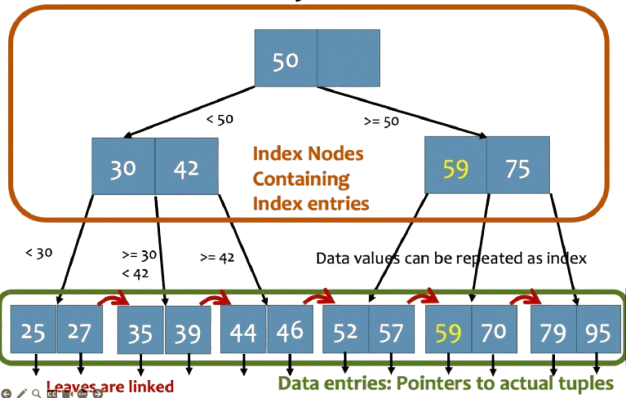
\includegraphics[scale=0.4]{img/bp_tree.png} 
        \caption{Note that the 59, which represents both the index and the data value, are repeated. In here, we assume a block size of 2. The leaf nodes are the indices that point to the tuples in the disk/memory. Sometimes, we may store the tuple directly in the nodes, which saves us another level of indirection, but this may cause memory problems if the tuples have too many attributes.} 
        \label{fig:bp_tree} 
      \end{figure}

      It has the following constraints. 
      \begin{enumerate}
        \item The \textbf{fanout} refers the to maximum number of pointers that can come out of each node. 
        \begin{figure}[H]
          \centering 
          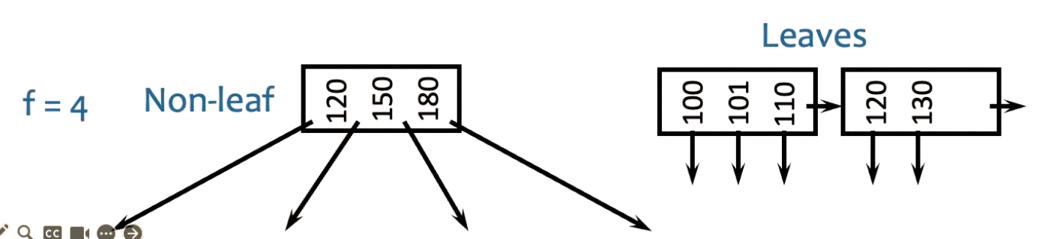
\includegraphics[scale=0.3]{img/fanout.png}
          \caption{With fanout constraint 4, for index nodes, we have 3 values with 4 pointers representing each range. For the leaves, we have 3 pointers to the disk addresses plus 1 pointer to the next node. } 
          \label{fig:fanout}
        \end{figure}

        \item The root is the only node that can store one value. It is special in this way. 
      \end{enumerate}
    \end{definition}

    Therefore, if we have a fanout of $f$, the table shows the constraints. 

    \begin{figure}[H]
      \centering 
      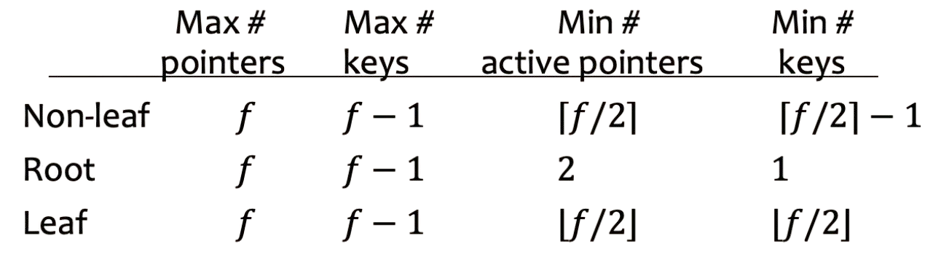
\includegraphics[scale=0.3]{img/chart.png}
      \caption{Note that there is a minimum constraint to ensure that the tree is balanced. } 
      \label{fig:chart}
    \end{figure}

    Now let's describe the implementation behind its supported operations. 

    \begin{algo}[Lookup]
      If we query \texttt{SELECT * FROM R WHERE k = 179;}, we go through the B+ tree's indices and reach the leaf node. From here, we can use the pointer to go to the memory address holding this tuple in memory/disk. If we query \texttt{k = 32}, then we will not find it after reaching \texttt{35}. If we want to query a range \texttt{32 < k < 179}, we start at 32 and use the leaf pointers to go to the next leaf until we hit 179.  

      \begin{figure}[H]
        \centering 
        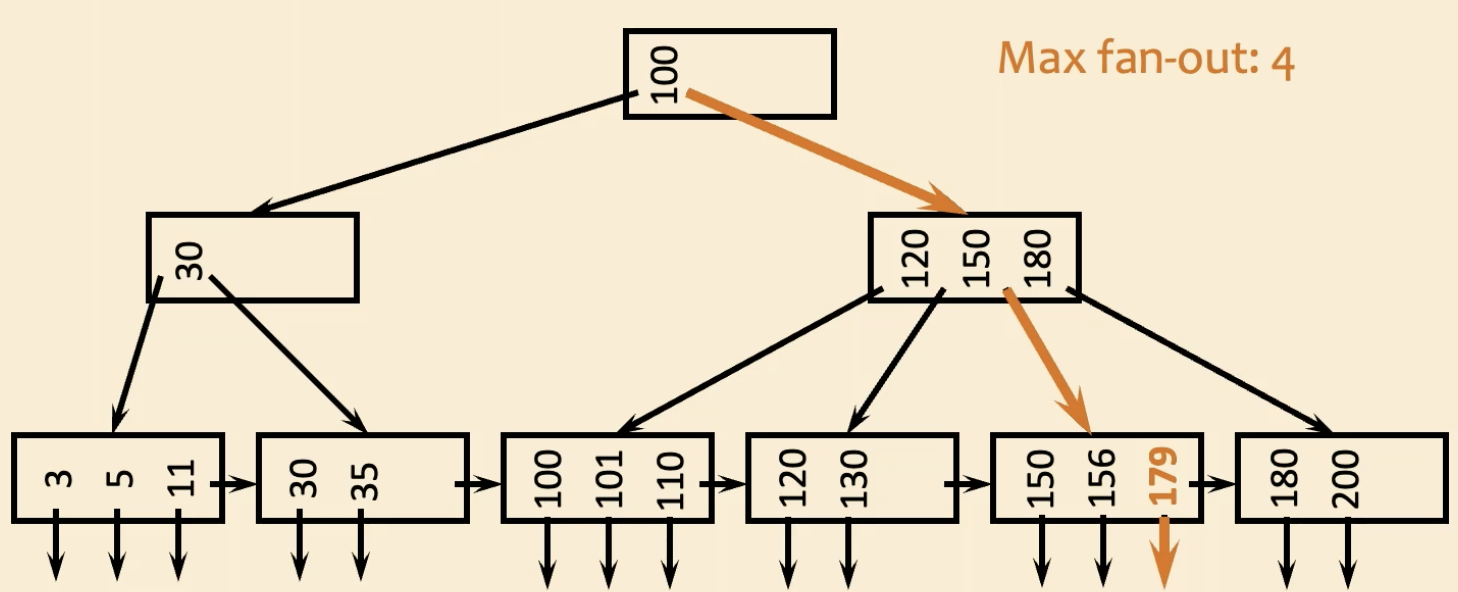
\includegraphics[scale=0.4]{img/fanout_ex.png}
        \caption{} 
        \label{fig:fanout_ex}
      \end{figure}

      In practice, there are much more pointers, so we could start at 179 and go back to 32 if we had backwards pointers. 
    \end{algo}

    \begin{algo}[Insertion]
      Insertion onto a leaf node having space is easy. 
      
      \begin{figure}[H]
        \centering 
        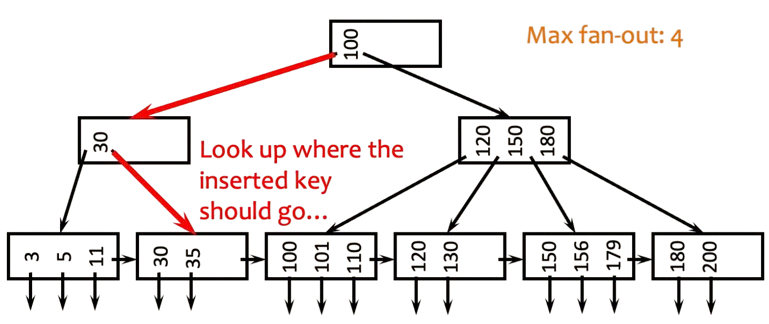
\includegraphics[scale=0.4]{img/insertion_easy.png}
        \caption{Note that to traverse this tree, we had to access 3 blocks of memory since for each block, we had to go to the disk, look up its contents, and retrieve the index of the next block (retrieve the blocks containing (100), (30), and (30, 35)) Then we have to update this block of (30, 35) and flush it. }
        \label{fig:insertion_easy}
      \end{figure}

      When we have a full node, it is more complicated. 
      \begin{enumerate}
        \item Say that we have a full node. We can try to push the rest of the leaf nodes to next node having space, but we are not guaranteed that the neighbors will have space. 

        \begin{figure}[H]
          \centering 
          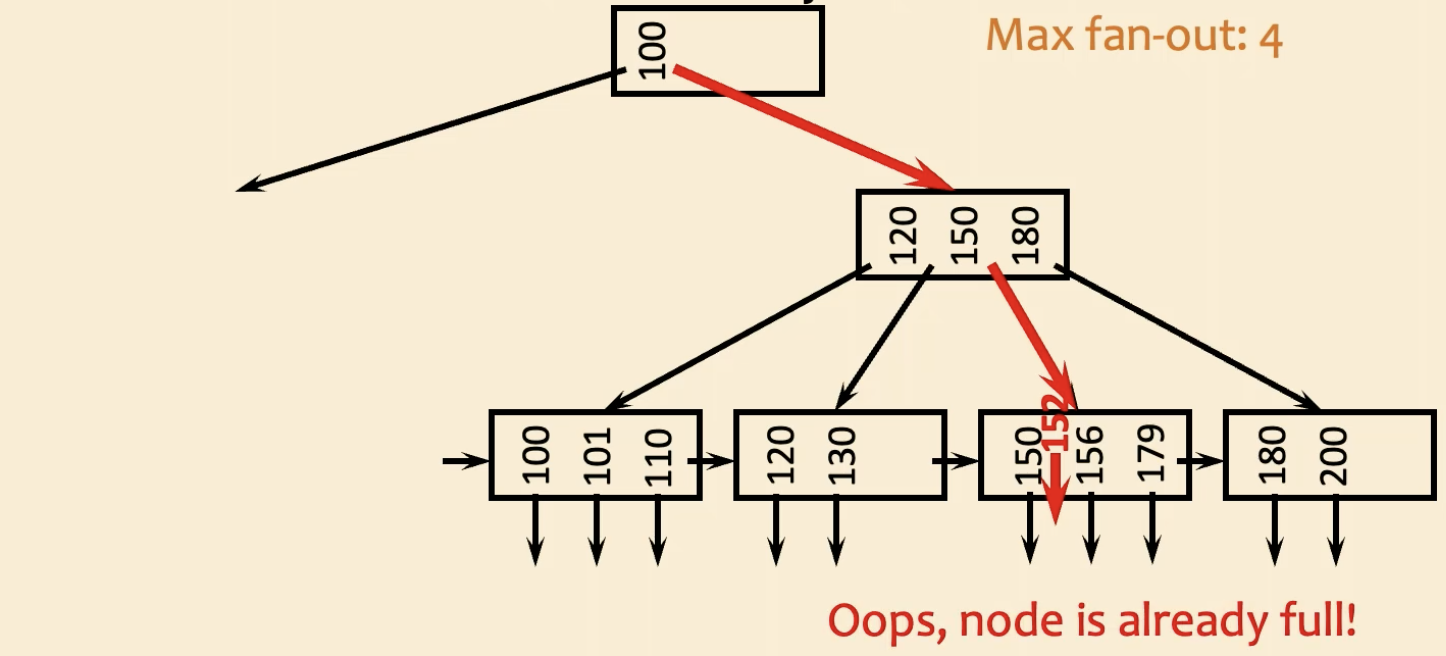
\includegraphics[scale=0.4]{img/insertion_1.png}
          \caption{} 
          \label{fig:insertion_1}
        \end{figure}

        \item We can split the node, called a \textbf{copy-up}. However, this new node now has no pointer. If the parent node is not full, we can just add the pointer and update its value. 

        \begin{figure}[H]
          \centering 
          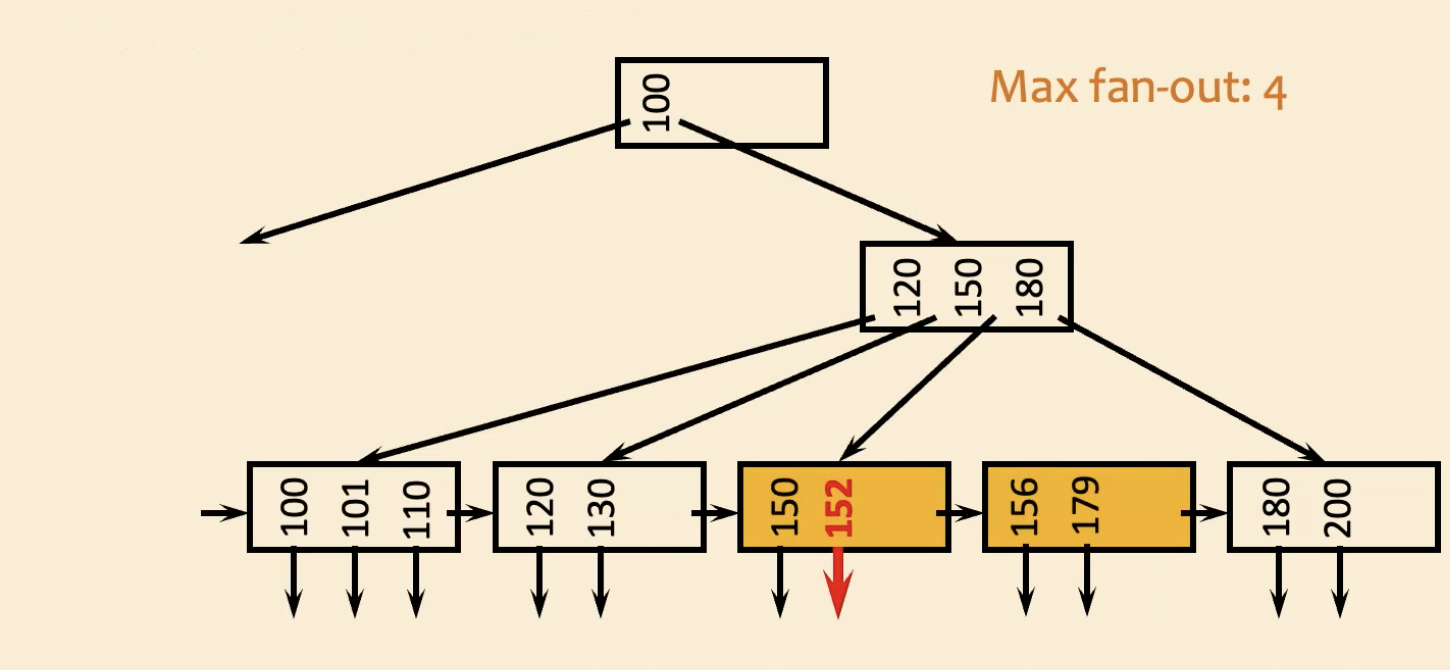
\includegraphics[scale=0.4]{img/insertion_2.png}
          \caption{} 
          \label{fig:insertion_2}
        \end{figure}

        \item If it is full, then we should split the parent node as well. This is called a \textbf{push-up}. 

        \begin{figure}[H]
          \centering 
          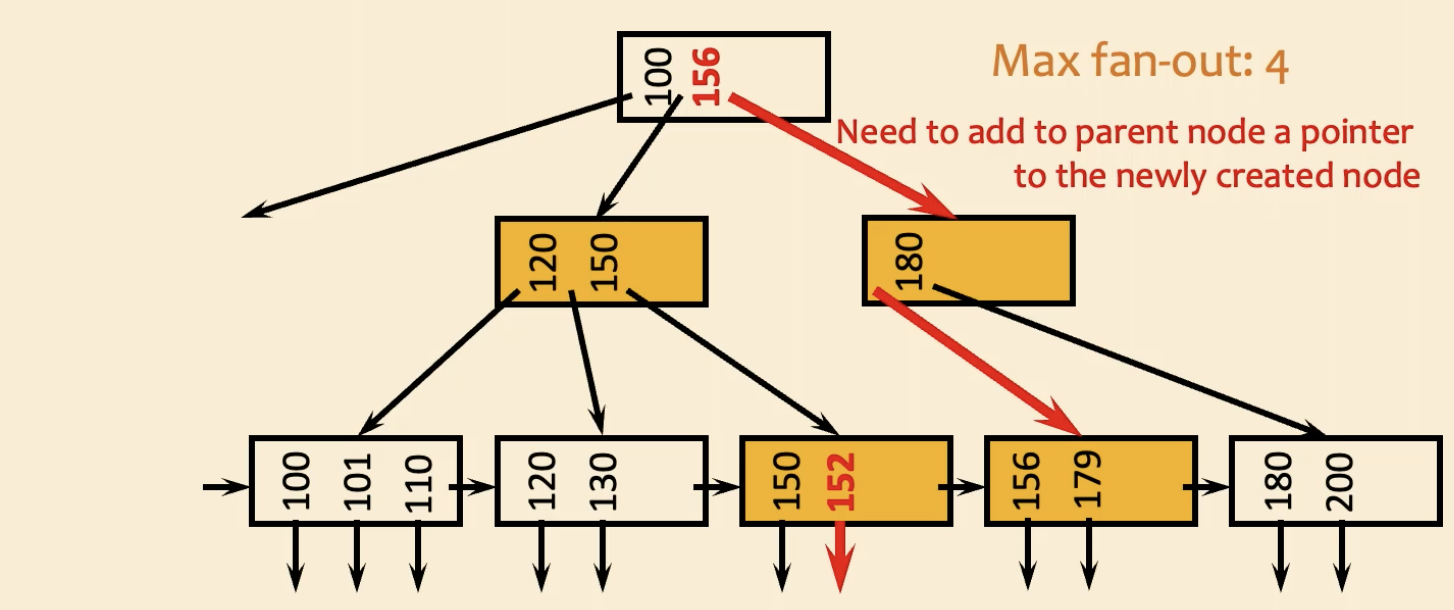
\includegraphics[scale=0.4]{img/insertion_3.png}
          \caption{} 
          \label{fig:insertion_3.png}
        \end{figure}

        \item This means that we have to update the parent of the parent. If the parent is not full, then we simply add it, and if it is full, then we split the parent of the parent, and so on. If we reach the root node, then we just split the root and increase the height of the tree.\footnote{This is rare in practice since the fanout is much greater than 3.}
      \end{enumerate}
    \end{algo}

    \begin{algo}[Deletion]
      Deleting a value is simple if after deletion, the leaf node has at least $f/2$ pointers ($f/2 - 1$ values). 
      
      \begin{enumerate}
        \item If the node has less than $f/2$ pointers, then it is too empty. We can adjust by taking adjacent nodes and moving them from the full nodes to the empty nodes, but this may steal too much from siblings. 

        \begin{figure}[H]
          \centering 
          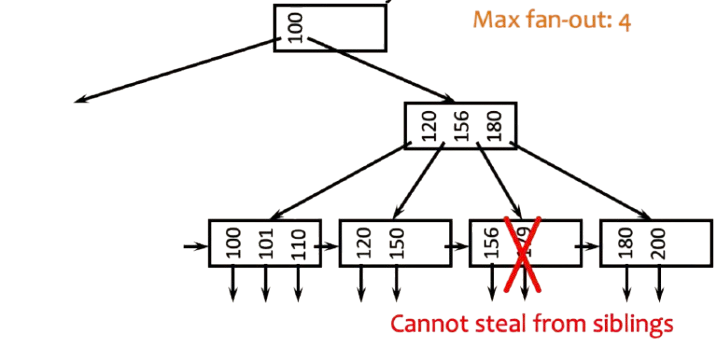
\includegraphics[scale=0.4]{img/deletion_1.png}
          \caption{} 
          \label{fig:deletion_1}
        \end{figure}

        \item The adjacent nodes may be empty as well, and in this case we want to \textbf{coalesce} or merge the nodes together. This results in a dangling pointer, so we delete the pointer and remove a value from the parent node.\footnote{In practice, this is not done every deletion. This reorganizing process can be deferred and the B+ tree property may temporarily not hold.} 

        \begin{figure}[H]
          \centering 
          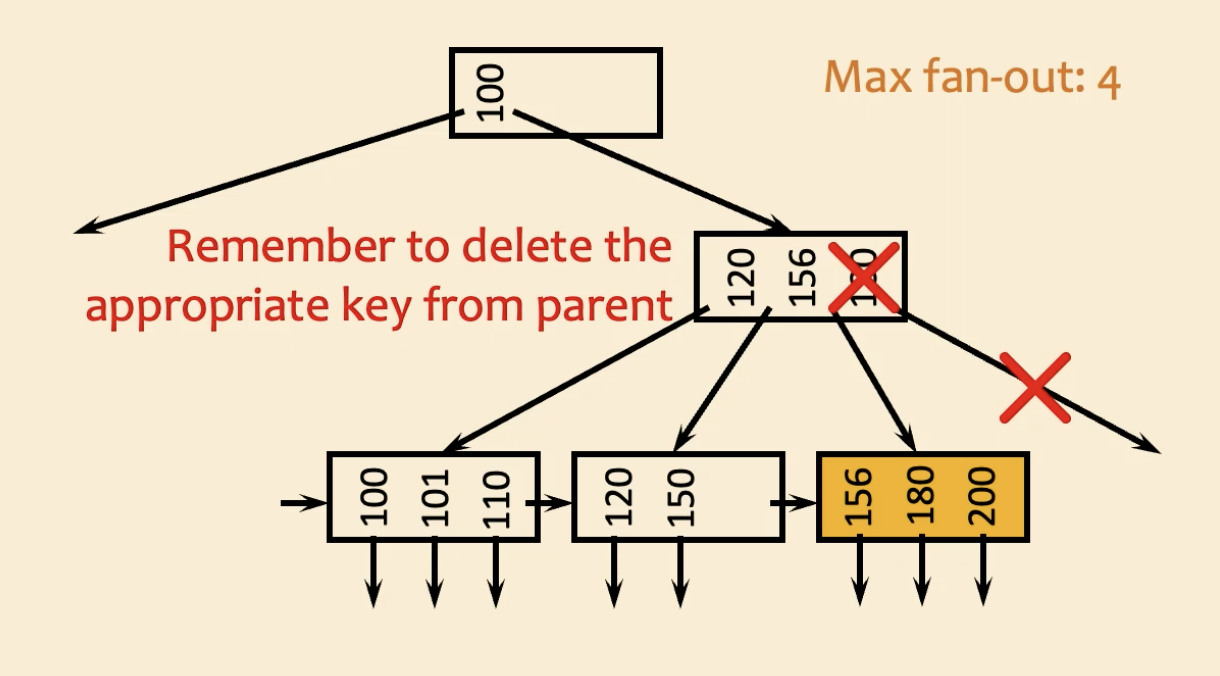
\includegraphics[scale=0.4]{img/deletion_2.png}
          \caption{} 
          \label{fig:deletion_2}
        \end{figure}

        \item We keep doing this until the B+ tree requirements are satisfied or we reach the root, at which point we delete the root node and our B+ tree height decreases by 1. 
      \end{enumerate}
    \end{algo}

    \begin{theorem}[IO Cost of Lookup, Insertion, Deletion]
      In general, all these operations have similar runtimes: 
      \begin{enumerate}
        \item They require us to go to the bottom of the tree, so it is $h$ operations, where $h$ is the height. 
        \item We also maybe have $+1$ or $+2$ to manipulate the actual records, plus $O(h)$ for reorganization like we saw before (which is rare if $f$ is large). 
        \item Minus 1 if we cache the root in memory, which can be decreased even further if we cache more blocks. 
      \end{enumerate}
      
      The actual size of $h$ is roughly $\log_{f/2} {N}$, where $N$ is the number of records. $f$ is the fanout, but the B+ tree properties guarantee that there are at least $f/2$ pointers, so it is $\log_{f/2} N$ at worst and $\log_{f} N$ at best. $f$ is very large usually so this is quite good. 
    \end{theorem}
    
    The reason we use B+ trees rather than B trees is that if we store data in non-leaf nodes, this decreases the fanout $f$ and increases $h$. Therefore, records in leaves require more I/Os to access. 

  \subsubsection{Clustered vs Unclustered Index} 

    Note that in a B+ tree, the leaf nodes always store the index in sorted order. This is so we can have fast lookup in indices. When we go into the disk, however, we may not have this assumption.  

    \begin{definition}[Clustered vs Unclustered Index]
      If the order of the data records on disk is the same as or close to the order of data entries in an index, then it is \textbf{clustered}, and otherwise \textbf{unclustered}. 

      \begin{figure}[H]
        \centering 
        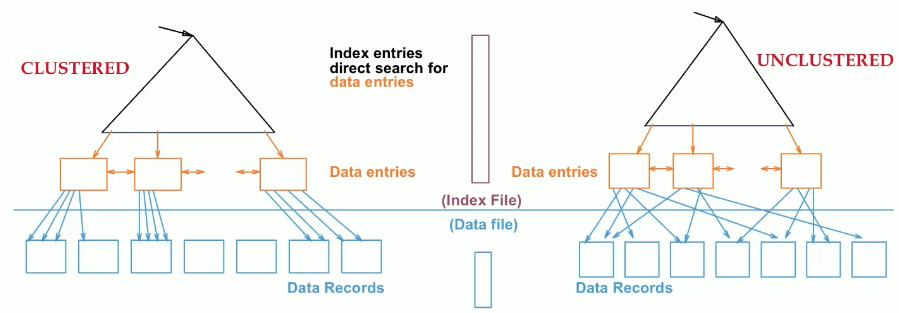
\includegraphics[scale=0.4]{img/clustered_vs_unclustered.png}
        \caption{Even if the data entries (leaf nodes) are sorted, the memory addresses of the blocks on disk that they point to may not be sorted.} 
        \label{fig:clustered_vs_unclustered}
      \end{figure}

      Note that the B+ tree is still a search tree! It is sorted. The clustered is a property of the data on disk (blue squares). 
    \end{definition}

    The performance can really depend on whether the index is clustered or unclustered. 

\subsection{Hash and Composite Index}

  \begin{definition}[Hash Index]
    So far, we have used tree indices. However, an alternative is to use a \textbf{hash index} which hashes the search keys for comparison. Hash indices can only handle equality queries. 
    \begin{enumerate}
      \item \texttt{SELECT * FROM R WHERE age = 5; } (requires hash index on \texttt{(age)})
      \item \texttt{SELECT * FROM R, S WHERE R.A = S.A; } (requires hash index on \texttt{R.A} or \texttt{S.A})
      \item \texttt{SELECT * FROM R WHERE age = 5 AND name = 'Bob' } (requires hash index on \texttt{(age, name)})
    \end{enumerate}
    They are more amenable to parallel processing but \textit{cannot handle range queries or prefixes}, e.g. \texttt{SELECT * FROM R WHERE age >= 5;}. Its performance depends on how good the hash function is (whether it distributes data uniformly and whether data has skew). 
  \end{definition}

  \begin{definition}[Composite Index]
    We've looked at queries in the form \texttt{SELECT \* FROM User WHERE age = 50;}, but what if there are multiple conditions. For example, if we have 
    \begin{lstlisting}
      SELECT * FROM User WHERE age >= 25 AND name = 'B'; 
    \end{lstlisting}
    then we can do a couple things: 
    \begin{enumerate}
      \item We have the index on \texttt{(age)}, at which point the leaf nodes will look something like 
        \begin{equation}
          25, 25, 25, 26, 26, 28, 29, 29
        \end{equation}
        We traverse through all the addresses in these leaf nodes and find the ones with name \texttt{B}. 

      \item If we have a \textbf{composite index} on \texttt{(age, name)}, then our leaf nodes will sort them as 
        \begin{equation}
          (25, A), (25, A), (25, B), (26, A), (26, C), (28, B), (29, A), (29, C)
        \end{equation}

      \item If we index on \texttt{(name, age)}, then our leaf nodes will sort them as 
        \begin{equation}
          (A, 25), (A, 25), (A, 26), (A, 29), (B, 25), (B, 28), (C, 26), (C, 29)
        \end{equation}
        Note that if we had the query \texttt{SELECT \* FROM R WHERE age >= 25}, then this sorting would not help since we do not prioritize ordering by age. So we cannot use tree indexing over name, age for this query. 
    \end{enumerate}
  \end{definition}

  \begin{example}
    Therefore, given a query, there are certain indices that we can use or cannot use for it.
    \begin{enumerate}
      \item If we have a query \texttt{A >= 5}, 
        \begin{enumerate}
          \item Can use hash index in general.  
          \item Can use tree index in general. 
        \end{enumerate}

      \item If we have query \texttt{A >= 5}, 
        \begin{enumerate}
          \item Can use tree with index (A). 
          \item Can use tree with index (A, B). 
          \item Cannot use tree with index (B, A) since A is not prefix. 
        \end{enumerate}

      \item If we have query \texttt{A = 5},
        \begin{enumerate}
          \item Can use hash with index (A). 
          \item Can use tree with index (A). 
          \item Cannot use hash with index (A, B) since hashing this tuple does not allow us to compare to A or retrieve it. It is one-way and pseudo-random.   
          \item Can use tree with index (A, B). 
        \end{enumerate}

      \item If we have \texttt{A = 5 AND B = 7}, 
        \begin{enumerate}
          \item Can use hash with index (A, B). 
        \end{enumerate}
    \end{enumerate}
  \end{example}

  Each index has its pros and cons, so why not just use both tree and hash indices? The problem is that when we modify a relation on the disk, we need to update the index as well. Therefore, having too many indices requires us to update more and takes more disk space. 

  Okay, so we can't use too many indices, but are indices \textit{always} better than table scans? Not exactly. 
  
  \begin{example}[Table Scans Wins]
    Consider $\sigma_{A > v} (R)$ and a secondary, non-clustered index on $R(A)$ with around 20\% of $R$ satisfying $A > v$ (could happen even for equality predicates). We need to follow pointers to get the actual result tuples. 
    \begin{enumerate}
      \item IOs for scan-based selection is simply $B(R)$ (where we can retrieve multiple tuples in this block), while 
      \item IOs for index-based selection is the lookup-cost (to traverse down the tree) plus $0.2 |R|$ (since for each tuple, we do a IO lookup, retrieve it, and then have to retrieve the next tuple which is likely not in the same block)
    \end{enumerate}
    So table scan wins if a block contains more than 5 tuples since we might as well grab everything rather than look them up one by one. 
  \end{example}

  Thankfully, the query optimizer will make these decisions for you. 

\subsection{Index Only Plans}

  \begin{definition}[Index-Only Plans]
    There are queries that can be answered only by accessing the index pages and not the data pages, known as \textbf{index-only plans}. For index-only plans, clustering is not important since we are looking only at the leaf nodes at most. Therefore, we only need to compute the I/O cost of traversing the tree and not to access data. 

    For equality, we can just compute the number of tuples in the index pages where the equality condition is satisfied. For ranges, we may need to traverse the leaf nodes, which will lead to additional I/O cost to retrieve the leaf index pages. 
  \end{definition}

  \begin{example}[Index Only Queries]
    If we look at the following query 
    \begin{equation}
      \pi_A (\sigma_{A > v} (R))
    \end{equation}
    we see that we only care about the value of $A$ and not the rest of the tuples, so we only need to look at the index pages and not the data itself. 
  \end{example}

  \begin{example}[Primary Index Clustered According to Search Key]
    If we have a primary index, in most cases the actual records are also stored in the index pages/leaf nodes. If they are clustered according to attribute $A$, then one lookup can lead to all result tuples in their entirety. You can just hit a leaf and grab your records as you walk along the leaves. 
  \end{example}

  \begin{example}[Other Index-Only Queries]
    For example, if we just wanted to look at the count of users with age 50, then we don't need the data. We can just look at the number of values in the leaf nodes of the B+ tree with this value. 
    \begin{lstlisting}
      SELECT E.do COUNT(*) 
      FROM Emp E 
      GROUP BY E.dno;
    \end{lstlisting}

    If we have an index on \texttt{(E.dno, E.sal)}, then the two queries are also index-only plans. However, if we index on \texttt{(E.dno)}, then we need to retrieve \texttt{E.sal} on the data page, incurring more cost. 

    \noindent\begin{minipage}{.5\textwidth}
    \begin{lstlisting}[]{Code}
      SELECT E.dno, MIN(E.sal) 
      FROM Emp E 
      GROUP BY E.dno; 
    \end{lstlisting}
    \end{minipage}
    \hfill
    \begin{minipage}{.49\textwidth}
    \begin{lstlisting}[]{Output}
      SELECT AVG(E.sal) 
      FROM Emp E 
      GROUP BY E.dno;
    \end{lstlisting}
    \end{minipage}
  \end{example}

  \begin{example}[Halloween Problem]
    The Halloween problem refers to a phenomenon in databases where an update operation causes a change in the physical location of a row, potentially allowing the row to be visited again later in the same update operation. Look at the update. 
    \begin{lstlisting}
      UPDATE Payroll 
      SET salary = salary * 1.1 
      WHERE salary <= 25000;
    \end{lstlisting}
    This caused everyone to have a salary of $25000+$. This is because when we updated someone with salary of say $1000$, it went to $1100$ and is moved further right in the B+ tree. Therefore, this is revisited again is increased again in the same update. To fix this, we could update the values in reverse, from the rightmost leaf node to the leftmost one so that increasing values are visited once. Or we can just create a to-do/done list that keeps track of which ones have been updated. 
  \end{example}

\subsection{Exercises}

  Now let's go through a bunch of questions to clarify some of the IO cost computation. 

  \begin{example}
    Assume that we have the query \texttt{SELECT * FROM User WHERE age = 50;} with the following assumptions: 
    \begin{enumerate}
      \item Assume 12 Users with \texttt{age = 50}. 
      \item Assume one data page (block) can hold 4 User tuples (so $f = 5$). 
      \item Suppose searching for data entry requires 3 IOs in a B+ tree, which contain pointers to the data records (so $h = 3$). 
    \end{enumerate}

    If the index is clustered, then we can just traverse down the B+ tree to get to the leaf node containing the value 50. 
    \begin{enumerate}
      \item We have a cost of 3 to traverse down the tree to access the index pages which show the memory addresses of the tuples on disk. 

      \item Then, we will find entries and we want to find the cost to access the data pages. There are 12 Users, and for every address, we load the entire block in memory, which will retrieve the other users of age 50 (since this is clustered). At best, we will retrieve 3 blocks (of 4 tuples each) and at worst, due to block overlap, we will retrieve 4 blocks and read the rest from memory. This gives us a cost of $+3$ or $+4$. 
    \end{enumerate}
    The total cost is 6. If the index is unclustered, then we are not guaranteed that the data with values 50 will be contiguous, so we will in the worst case have to look at 12 different blocks, leading to a total cost of $3 + 12 = 15$. 
  \end{example}

  \begin{example}[Index Problem]
    Consider a table \texttt{Orders(OrderID, CustomerID, OrderDate, TotalAmount)} with 5,000,000 records stored in 100,000 disk blocks (=pages or units of I/O). The rows are not sorted on any particular attribute. There is a \textbf{clustered} B+ tree index on OrderID (the primary key), and an \textbf{unclustered} B+ tree index on CustomerID.

    Assume the following:
    \begin{itemize}
      \item Each node in the B+ trees corresponds to one disk block.
      \item The OrderID B+ tree has 4 levels (including the root) and 10,000 leaf nodes.
      \item The CustomerID B+ tree has 5 levels (including the root) and 50,000 leaf nodes.
      \item You do not have enough space in memory to hold all data pages.
      \item The root nodes of both B+ trees are always kept in memory.
      \item The non-root index nodes and all data pages are initially on disk.
      \item All the leaves have pointers to the next left node both on the left and the right side.
      \item All data pages are fully utilized.
      \item All nodes in B+ trees are also fully utilized.
      \item Uniformity in all places. You can ignore page boundaries.
    \end{itemize}

    \noindent\textbf{Question 1.1}\\
    How many disk I/Os are required (index and data) to retrieve all order records for a specific CustomerID using the index on the CustomerID? Assume there are 100 orders for this customer.

    We must access 4 levels, with 5 levels in tree minus 1 for head already in memory (+4). There is only 1 leaf index pages containing the matching entries, since there are 5m records and 50k leaf nodes, meaning that each leaf node can contain 100 addresses at most when it is a dense index. Given that there are 100 matches, we just need to use this leaf node to access the disk. This is not clustered, so we must look through all 100 addresses, reading each block from disk for an addition cost of 100 IOs. Total is \textbf{104 IOs}. 

    \vspace{1em}
    \noindent\textbf{Question 1.2}\\
    Suppose the Orders table is frequently queried for recent orders, and the performance is critical. The current clustered index on OrderID is not providing optimal performance for these queries. You are considering reorganizing the Orders table to cluster it on OrderDate instead.

    Assume that orders are uniformly distributed over time. Everything else is the same as in the original question description \textbf{(i.e., the number of levels of the new B+ tree indexed on OrderDate is still 4 and the root is still in memory. And the number of leaf nodes is still 10,000)}. Ignore page boundaries.

    Consider the following query:
    \begin{lstlisting}
    SELECT * FROM Orders 
    WHERE OrderDate BETWEEN '2023-09-01' AND '2023-09-30';
    \end{lstlisting}

    How many disk I/Os are required in the worst case for the following query before and after the change? What is the impact of the change? Assume that 0.5\% of the orders were made in September 2023.

    For before, since the data is distributed uniformly, we must in the worst case check all data pages of the relation on disk. 
    \begin{enumerate}
      \item We first have 3 IOs to go down to the leaf (4 levels minus 1 head already in memory). 
      \item We scan through all 10,000 leaves, but we are already on leaf 1, so need to traverse 9999 pointers to load each index leaf. 
    \end{enumerate}
    Therefore, the total IO for traversal is \textbf{10,002 IOs}. If we include the IOs for loading data pages, we also incur more costs. There are 100,000 disk blocks, so as we load all of them we incur an additional IO cost of 100,000, giving us \textbf{110,002 IOs}. 


    For after, if we cluster on OrderDate, then out of the 100,000 disk blocks, we assume that 0.5\% of them, or 500 of them, will contain the relevant dates. Additionally, we assume that by uniformity, 0.5\% of the 10,000 leaf nodes will contain these relevant addresses. 
    \begin{enumerate}
      \item We traverse down to the leaf containing the address of the tuple with date attribute \texttt{2023-09-01}. This is 3 IOs. 
      \item We must traverse through the rest of the leaf nodes. Since we are already at the first one, we must load in an additional 49 leaf blocks, so 49 IOs. 
      \item As we load in each block, we are loading in a total of 500 data blocks from disk, so an additional 500 IOs. 
    \end{enumerate}
    We end up with \textbf{552 IOs}. If we exclude the IOs for loading the data pages, we incur fewer cost of \textbf{52 IOs} since this is only for traversal of the B+ tree. 

    The difference in these costs is just the first value minus the second value. For example, I can do 
    \begin{equation}
      10,002 - 552 = 9450
    \end{equation}
    reduced IO costs. 


    \vspace{1em}
    \noindent\textbf{Question 1.3}
    \begin{enumerate}[label=(\alph*)]
      \item How many disk I/Os are required in the worst case to insert a new order with order ID 2000 and customer ID 200 if updating the clustered index on the Order ID? (i.e., what is the I/O required for updating the index and inserting data records?)
      \item What would the result be if we updated the unclustered index on the CustomerID?
    \end{enumerate}

    Assume all memory blocks are being used for this update only. Then we do not throw away an index page once it is read.

    For (a), 
    \begin{enumerate}
      \item You should first get 3 IOs to traverse down to the leaf. 
      \item Then you load the relevant data page from disk onto memory (1 IO). 
      \item Since this block is full and you want to add a tuple to it, you must split it into two pages. So you initialize two buffers in memory and write two separate blocks. Then you must write these blocks back into disk (2 IOs). 
      \item Then you split the leaf (assuming it's already in memory) by writing its 2 splits back, again by splitting it in memory (2 IOs). You this for the next node (since in worst case it's full), for a total of 3 more times as you traverse up the tree (6 IOs). 
      \item You finally want to write a new root into the disk, so you make one in memory and write it (1 IO). 
    \end{enumerate}
    This gives a total of \textbf{15 IOs}. 

    For (b), should be 17 or 18? 
    \begin{enumerate}
      \item You should first traverse down to the leaf (+4 IOs). 
      \item Then you take a data page and write it in memory (+1 IO) since you don't need to split it to keep the clustering. Then you flush the new page to disk (+2 IOs). 
      \item Then you split the leaf node by writing its 2 splits back (+2). You do this 4 more times (+8 IOs). 
      \item You then want to write a new root node (+1). So in total +16 IOs. 
    \end{enumerate}
  \end{example}

